\chapter{Veje og Kredse}



\section{Veje}
Veje i en graf viser, hvilke ruter der er rundt i en graf. Dette er relevant for at finde ruter til en GPS, et computernetværk eller andet, hvor der er behov for at bestemme en rute gennem flere steder. 
En vej i en graf defineres i Definition \ref{def_vej}.

\begin{defn}
\label{def_vej}
Lad $n \in  \mathbb{Z}^{+}$ og lad $G$ være en ikke-orienteret graf. 
En \textit{vej} af \textit{længde} $n$ fra $u$ til $v$ i $G$ er en sekvens af $n$ kanter $e_1, ..., e_n$ i $G$, for hvilke der eksisterer en sekvens $x_0=u,x_1,...,x_{n-1},x_n=v$ af punkter, så $e_i$ har endepunkterne $x_{i-1}$ og $x_1$ for $i=1,...,n$.
\end{defn}

\noindent Når der er tale om en vej gennem en simpel graf, noteres denne som sekvensen af de knuder, den går igennem $x_0, x_1,...,x_n$. 
En vej eller kreds er \textit{simpel} hvis den ikke indeholder den samme kant mere end én gang. 

\begin{exmp}
\label{ex_vej}
På den simple graf i Figur \ref{graf_vej} ses en simpel vej $A,B,E,F$ af længden 3, fordi vejen går gennem de tre kanter $\lbrace A,B \rbrace$, $\lbrace B,E \rbrace$ og $\lbrace E,F \rbrace$. 
Vejen er simpel, fordi den ikke går gennem den samme kant mere end en gang. 
Derimod er $A,B,D,E$ ikke en vej, fordi $\lbrace B,D \rbrace$ ikke er en kant. 
Vejen $A,B,C,E,B,A$ er også en vej, men den er ikke simpel, fordi den går gennem kanten $\lbrace A,B \rbrace$ to gange. 
\end{exmp}

\begin{figure}[h]
\centering
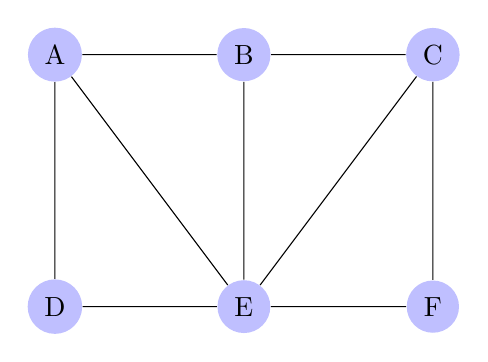
\begin{tikzpicture}
[scale=.8,auto=left,every node/.style={circle,fill=blue!25}]
  \node (n6) at (3,2) {D};
  \node (n4) at (3,6) {A};
  \node (n5) at (6,2) {E};
  \node (n1) at (6,6) {B};
  \node (n2) at (9,2) {F};
  \node (n3) at (9,6) {C};
  \foreach \from/\to in {n6/n4,n4/n5,n5/n1,n2/n5,n2/n3,n3/n1,n1/n4,n6/n5,n5/n3}
    \draw (\from) -- (\to);
\end{tikzpicture}
\caption{graf} 
\label{graf_vej}
\end{figure}

\section{Kredse}
I et særligt tilfælde, kan en vej kaldes en kreds.
En kreds er en vej, der starter og slutter det samme sted, hvilket defineres i Definition \ref{def_kredse}

\begin{defn}
\label{def_kredse}
En vej er en \textit{kreds}, hvis den begynder og ender i samme punkt, $u=v$ og $n>0$.
Vejen eller kredsen siges at gå gennem punkterne $x_1,x_2,...,x_{n-1}$ eller passere gennem kanterne $e_1, e_2,...e_n$.
\end{defn}

\begin{exmp}
I Figur \ref{graf_kreds} ses en kreds, $A,B,C,E,D,A$, som har længden 5, fordi den går gennem 5 kanter. Det er en kreds, fordi den begynder og ender i punktet $A$.
I Figur \ref{graf_ikke_kreds} ses en vej $C,B,A,D,E,C,F$.
Denne vej er ikke en kreds, fordi den ikke starter og slutter i samme punkt. 
\end{exmp}

\begin{figure}[!htb]
   \begin{minipage}{0.48\textwidth}
     \centering
     	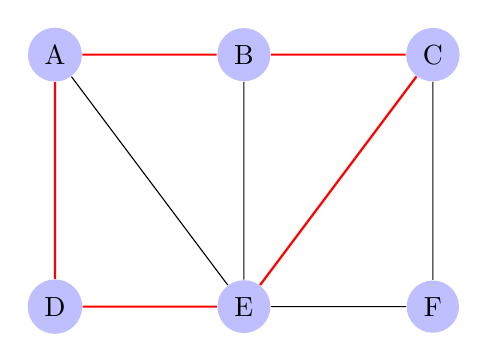
\begin{tikzpicture}
[scale=.8,auto=left,every node/.style={circle,fill=blue!25}]
  \node (n6) at (3,2) {D};
  \node (n4) at (3,6) {A};
  \node (n5) at (6,2) {E};
  \node (n1) at (6,6) {B};
  \node (n2) at (9,2) {F};
  \node (n3) at (9,6) {C};
  \draw (n6) edge [red, thick] (n4);
  \draw (n6) edge [red, thick] (n5);
  \draw (n5) edge [red, thick] (n3);
  \draw (n3) edge [red, thick] (n1);
  \draw (n1) edge [red, thick] (n4);
  \foreach \from/\to in {n5/n1,n2/n5,n2/n3,n4/n5}
    \draw (\from) -- (\to);
\end{tikzpicture}
     \caption{Kreds}
     \label{graf_kreds}
   \end{minipage}\hfill
   \begin{minipage}{0.48\textwidth}
     \centering
     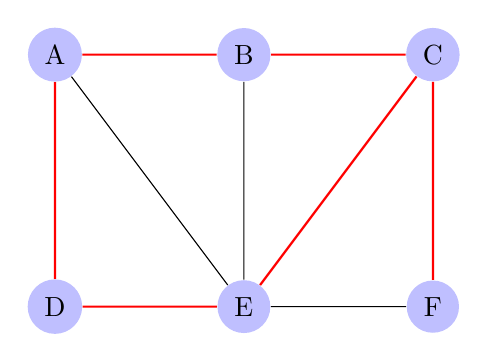
\begin{tikzpicture}
[scale=.8,auto=left,every node/.style={circle,fill=blue!25}]
  \node (n6) at (3,2) {D};
  \node (n4) at (3,6) {A};
  \node (n5) at (6,2) {E};
  \node (n1) at (6,6) {B};
  \node (n2) at (9,2) {F};
  \node (n3) at (9,6) {C};
  \draw (n6) edge [red, thick] (n4);
  \draw (n6) edge [red, thick] (n5);
  \draw (n5) edge [red, thick] (n3);
  \draw (n3) edge [red, thick] (n1);
  \draw (n1) edge [red, thick] (n4);
  \draw (n3) edge [red, thick] (n2);
  \foreach \from/\to in {n5/n1,n2/n5,n4/n5}
    \draw (\from) -- (\to);
\end{tikzpicture}
     \caption{Vej}
     \label{graf_ikke_kreds}
   \end{minipage}
\end{figure}

\section{Sammenhængende grafer}
For en graf kan det være relevant at afgøre, om der er en forbindelse mellem alle punkter i grafen, således, at det er miuligt at komme fra et hvilket som helst punkt til et andet. Dette bestemmes ud fra, om en graf er sammenhængende eller ej.
I dette kapitel vil der kun blive fokuseret på ikke-orienterede grafer.
En sammenhængende graf defineres i Definition \ref{def_iosmh}.

\begin{defn}
\label{def_iosmh}
En ikke-orienteret graf siges at være \textit{sammenhængende}, hvis der er en vej mellem hvert punktpar i grafen. 
En ikke-orienteret graf, der ikke er sammenhængende, kaldes \textit{ikke-sammenhængende}.
Det siges, at en graf opdeles, når punkter, kanter eller begge fjernes for at lave en undergraf. 
\end{defn}

\noindent På den måde ses det, at der i en sammenhængende graf findes en vej mellem alle punkter i grafen. 
Det er derfor muligt at komme fra et hvilket som helst punkt i grafen til et andet.

\begin{thm}
Der er en simpel vej mellem ethvert punktpar i en sammenhængende ikke-orienteret graf.
\label{smh_satning}
\end{thm}

\begin{proof}
Knuderne $u$ og $v$ er to knuder i den sammenhængende graf $G=(V,E)$.
Per Definition \ref{def_iosmh} er der en simpel vej mellem $u$ og $v$.
Lad den korteste vej mellem $u$ og $v$ være $x_0,x_1,...,x_n$, hvor $x_0=u$ og $x_n=v$.
Denne vej af kortest længde er simpel, fordi den ikke går gennem den samme kant flere gange. 
For at bevise det, antages det, at den ikke er simpel. 
Så er $x_i=x_j$ for $0 \leq i < j$.
Det betyder, at der er en kortere vej fra $u$ til $v$, med punktsekvens $x_0,x_1,...,x_{1-i},x_j,...,x_n$, som opnåes ved at fjerne kanterne i sekvensen $x_i,...,x_{j-1}$.
\end{proof}

\subsection{sammenhængsgrad}
Kommer senere

\section{Eulerkredse}

En bestemt type af kredse gennemgår alle kanter i en graf og kaldes Eulerkredse. 

\begin{defn}\label{euler_def}
En Eulerkreds er en simpel kreds i grafen $G$ som indeholder hver kant i $G$.
En Eulervej er en simpel vej i grafen $G$, som indeholder hver kant i $G$.  
\end{defn}
\begin{exmp}
Eksempler på en Eulerkreds og en Eulervejkan ses her: 
\end{exmp}

\begin{figure}[h]
\centering
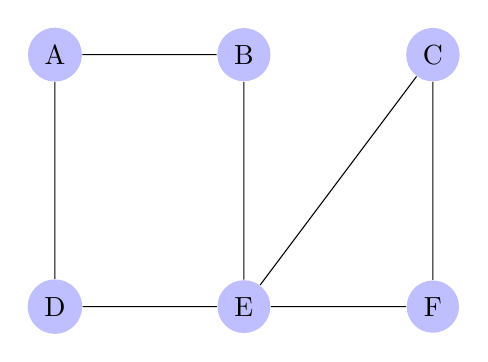
\begin{tikzpicture}
[scale=.8,auto=left,every node/.style={circle,fill=blue!25}]
  \node (n6) at (3,2) {D};
  \node (n4) at (3,6) {A};
  \node (n5) at (6,2) {E};
  \node (n1) at (6,6) {B};
  \node (n2) at (9,2) {F};
  \node (n3) at (9,6) {C};
  \foreach \from/\to in {n6/n4,n5/n1,n2/n5,n2/n3,n1/n4,n6/n5,n5/n3}
    \draw (\from) -- (\to);
\end{tikzpicture}
\caption{Euler kreds} 
\label{euler_kreds}
\end{figure}

\noindent Et eksempel på en Eulerkreds i Figur \ref{euler_kreds} kan være: $A,B,E,C,F,E,D,A$


\input{fig/tikz/euler_vej}

\noindent Et eksempel på en Eulervej i Figur \ref{euler_vej} kan være: $A,B,E,D,A,E,F,C$

\noindent Der eksiserer ikke en Eulerkreds i alle grafer. \\

For at der kan eksisere en Eulerkreds i en sammenhægende multigraf skal Sætning \ref{Eulerkreds_multigraf} gælde. 

\begin{thm}\label{Eulerkreds_multigraf}
En sammenhængende multigraf med mindst to knuder, har en Eulerkreds hvis og kun hvis, hver knude er af lige grad.
\end{thm}

\begin{proof} 
En kreds begynder i en knude $a$ og fortsætter langs en kant, som er incident med $a$, til en ny knude $b$. 
Denne kant kaldes $\lbrace a,b \rbrace$, kanten bidrager med 1 til $deg(a)$. 
Hver gang kredsen passere gennem en knude, tilføjes 2 til graden af denne knude. 
Til sidst ender kredsen tilbage i $a$, og bidrager igen med 1 til $deg(a)$. 
Derfor må $deg(a)$ være lige og graden af hver knude må også være lige.  
\end{proof} 

\noindent Det er muligt at lave en algoritme som kan finde en Eulerkreds i en multigraf.
En sådan algoritme vil første tage udgangspunkt i en tilfældig underkreds i graf G, hvorefter der indeføres en variabel H, som er lig med G, foruden kanterne i den tilfældige underkreds. 
Så længe H indeholder kanter, vil en løkke køre. 
Under denne løkke dannes en ny delkreds i H, hvor en af knuderne også skal være endepunkt for en kant i en tidligere underkreds.
Dernæst fjerns kanterne i underkredsen fra H sammen med enventuelt isolerede knuder. 
Til sidst sammensættes underkredsene til en samlet kreds, som retuneres.
Proceduren kan ses i Algoritme \ref{algoritme_euler}.
Der findes også andre algoritmer, som kan finde Eulerkredse i en graf, men disse bliver ikke nævnt i dette projekt.\\
  

\begin{algorithm}
\caption{Eulerkredse}
\label{algoritme_euler}
\textbf{procedure} Euler(G: sammenhængende mulitgraf med knuder af lige grad)\\
$kreds:=$ en kreds i G begynder i en vilkårlig knude med kanter, der danner en kreds.\\
$H:= G$ med kanterne fra $kreds$ fjernet\\
\textbf{når} $H$ har kanter\\
$\-$ $\-$ $\-$ $\-$ $\-$ $\-$
$underkreds:=$ en kreds i $H$, der begynder i en knude i $H$, som også er et endepunkt af en kant i $kreds$ \\ 
$\-$ $\-$ $\-$ $\-$ $\-$ $\-$
$H:=$ $H$ uden kanterne af $underkreds$ samt alle isolerede knuder fjernet \\
$\-$ $\-$ $\-$ $\-$ $\-$ $\-$
$kreds:=$ $kreds$ med $underkreds$ indsat ved den passende knude \\ 
\textbf{retuner} $kreds$ ($kreds$ er en Eulerkreds)
\end{algorithm}

$\-$ $\-$ $\-$ $\-$ $\-$ $\-$ \\
\noindent Hvis der ikke findes en Eulerkreds i en graf, kan der godt eksistere en Eulervej. 
For at der kan findes en Eulervej skal Sætning \ref{Eulervej_multigraf} gælde. 

\begin{thm} \label{Eulervej_multigraf}
En sammenhængende multigraf graf G har en Eulervej, men ikke en Eulerkreds, hvis og kun hvis den har præcist to knuder af ulige grad.  
\end{thm} 

\begin{proof}
Antag at en sammenhængende multigraf G har en Eulervej fra $a$ til $b$, men ikke en Eulerkreds. 
Den første kant som passeres på vejen bidrager med 1 til $deg(a)$. 
Hver gang vejen passerer knuden $a$ vil 2 tilføjes til $deg(a)$. 
Den sidste kant på vejen bidrager 1 til graden af endepunktet for vejen, $deg(b)$. 
Ligesom for $a$, kan vejen krydse $b$. 
Hver gang dette måtte ske tilføjes 2 til graden af $b$. 
Resultatet bliver, at $a$ og $b$ altid vil være af ulige grad. 
Alle andre knuder på vejen vil være af lige grad, fordi at 2 tilføjes til graden af en knude, hver gang en knude passeres.  
\end{proof}

